\subsection{Finite Field Dependency}
\label{sec:implementation__dependencies}
\label{sec:implementation_dependency}

An integral part of Elliptic Curve cryptography is finite field arithmetic. No implementation of finite field elements exists
in the standard libraries of .NET, so an external source must be used. BouncyCastle provides an implementation (\texttt{FpFieldElement})
that is repurposed and used in OpenECC.

The repurposing is not without problems. BouncyCastle uses a custom implementation of integers, to allow large integers to
be used, than the standard \texttt{System.Numerics.BigInteger}. Conversion between the two is non-trivial (especially as no documentation
of the internal structure of BouncyCastle's \texttt{BigInteger} exists).

The safest way of converting from \texttt{System.Numerics.BigInteger} to \\
\texttt{Org.BouncyCastle.Math.EC.BigInteger} is then to convert one to a string and get the other to parse said string. This conversion,
to and from string, is expected to be slow.

BouncyCastle's \verb+BigInteger.ToString+ method has a comment (in the source code) stating that ``[this] is algorithm 1a from chapter
4.4 in Seminumerical Algorithms, \textbf{slow but it works}'' (emphasis added). Avoiding any calls to this method drastically improved
performance. Having to convert integers from one representation to another fairly often is still expected to incur a performance
penalty.\footnote{The actual impact on performance is investigated in Section \ref{sec:performance_components_biginteger}.}

\begin{figure}[htb]
	\centering
	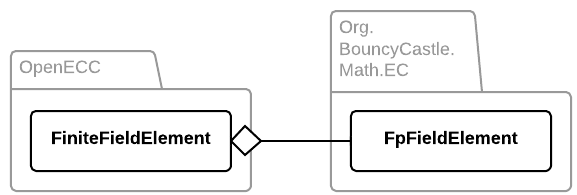
\includegraphics[width=0.7\textwidth]{implementation/finitefields}
	\caption{The \texttt{FiniteFieldElement} is simply a wrapper around \texttt{Org.BouncyCastle.Math.EC.FpFieldElement},
		BouncyCastle's Finite Field implementation.}
\end{figure}

OpenECC's \texttt{FiniteFieldElement} is a wrapper around BouncyCastle's \\
\verb+FpFieldElement+ and provides access to the necessary methods.
In addition to this, the \texttt{FiniteFieldElement} implementation also provides a nicer syntax for performing the necessary operations
(for the same reasons as doing so for \texttt{Point}s). This will make future implementations of other constructs, that rely on finite fields,
easier and more readable.